% Preamble
\documentclass[xcolor=dvipsnames]{beamer}
\usetheme{madrid}

% Packages
\usepackage[english,ngerman]{babel}
\usepackage[utf8]{inputenc}
\usepackage{amsmath}
\usepackage{graphicx}
\usepackage{ifthen} % Boolean variables
\usepackage{subfigure} % Horizontal pictures

\definecolor{hBlue}{RGB}{55,118,165}
\usecolortheme[named=hBlue]{structure}

% Distiction between work and stream presentation
\newboolean{work}
\setboolean{work}{true}

\ifthenelse{\boolean{work}}{
    \titlegraphic{
\includegraphics[width=4cm]{../images/logo.png}}
}{}
\title{Gesundheit \& Ernährung}
\subtitle{Makronährstoffe II: Fette}
\ifthenelse{\boolean{work}}{
    \author{Adrian Helberg}
}{
    \author{Bl1nzlar, twitch.tv/bl1nzlar}
}
\date{30.06.2021}


% Document
\begin{document}

    \maketitle

    \frame{\frametitle{Agenda}\tableofcontents}

    \section{Theorie}
    {
    \setbeamercolor{normal text}{fg=hBlue}\usebeamercolor*{normal text}
    \begin{frame}
        \begin{center}
            \Huge Theorie
        \end{center}
    \end{frame}
    }

    \subsection{Profil}
    \begin{frame}[allowframebreaks]
        \frametitle{Fett im Profil}

        \begin{figure}
            \centering
            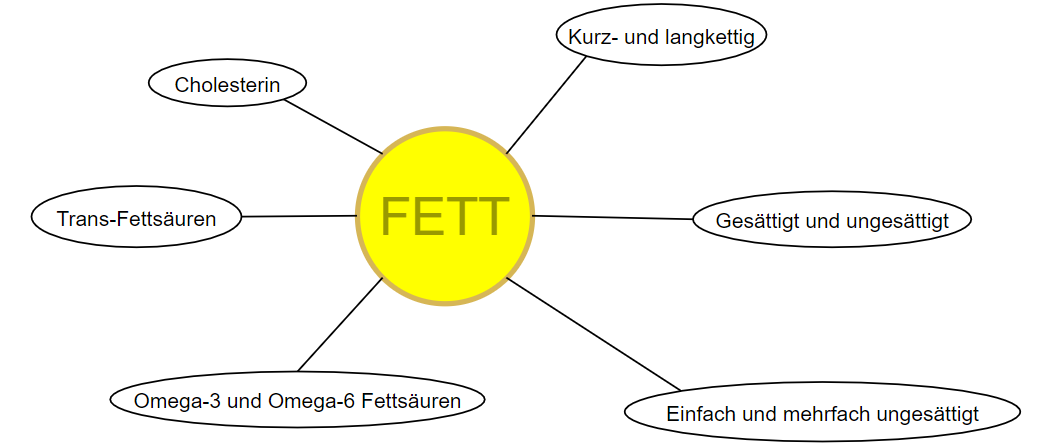
\includegraphics[width=10cm]{../images/fett.png}
            \caption{Schlagworte in Verbindung mit Fett}
        \end{figure}

        \framebreak

        \begin{block}{Was ist Fett?}
            \begin{itemize}
                \setlength\itemsep{1em}
                \item Fettsäuren als kleinste Bausteine von Fett
                \item Die meisten Fettsäuren können (wie Traubenzucker) in den meisten Zellen des Körpers zu Energie verbrannt werden
                \item Einige Fettsäuren können in großen Mengen im Fettgewebe gespeichert werden
                \item Manche Fettsäuren werden als Baustoff für bspw. Zellwende benötigt
            \end{itemize}
        \end{block}

        \begin{figure}
            \centering
            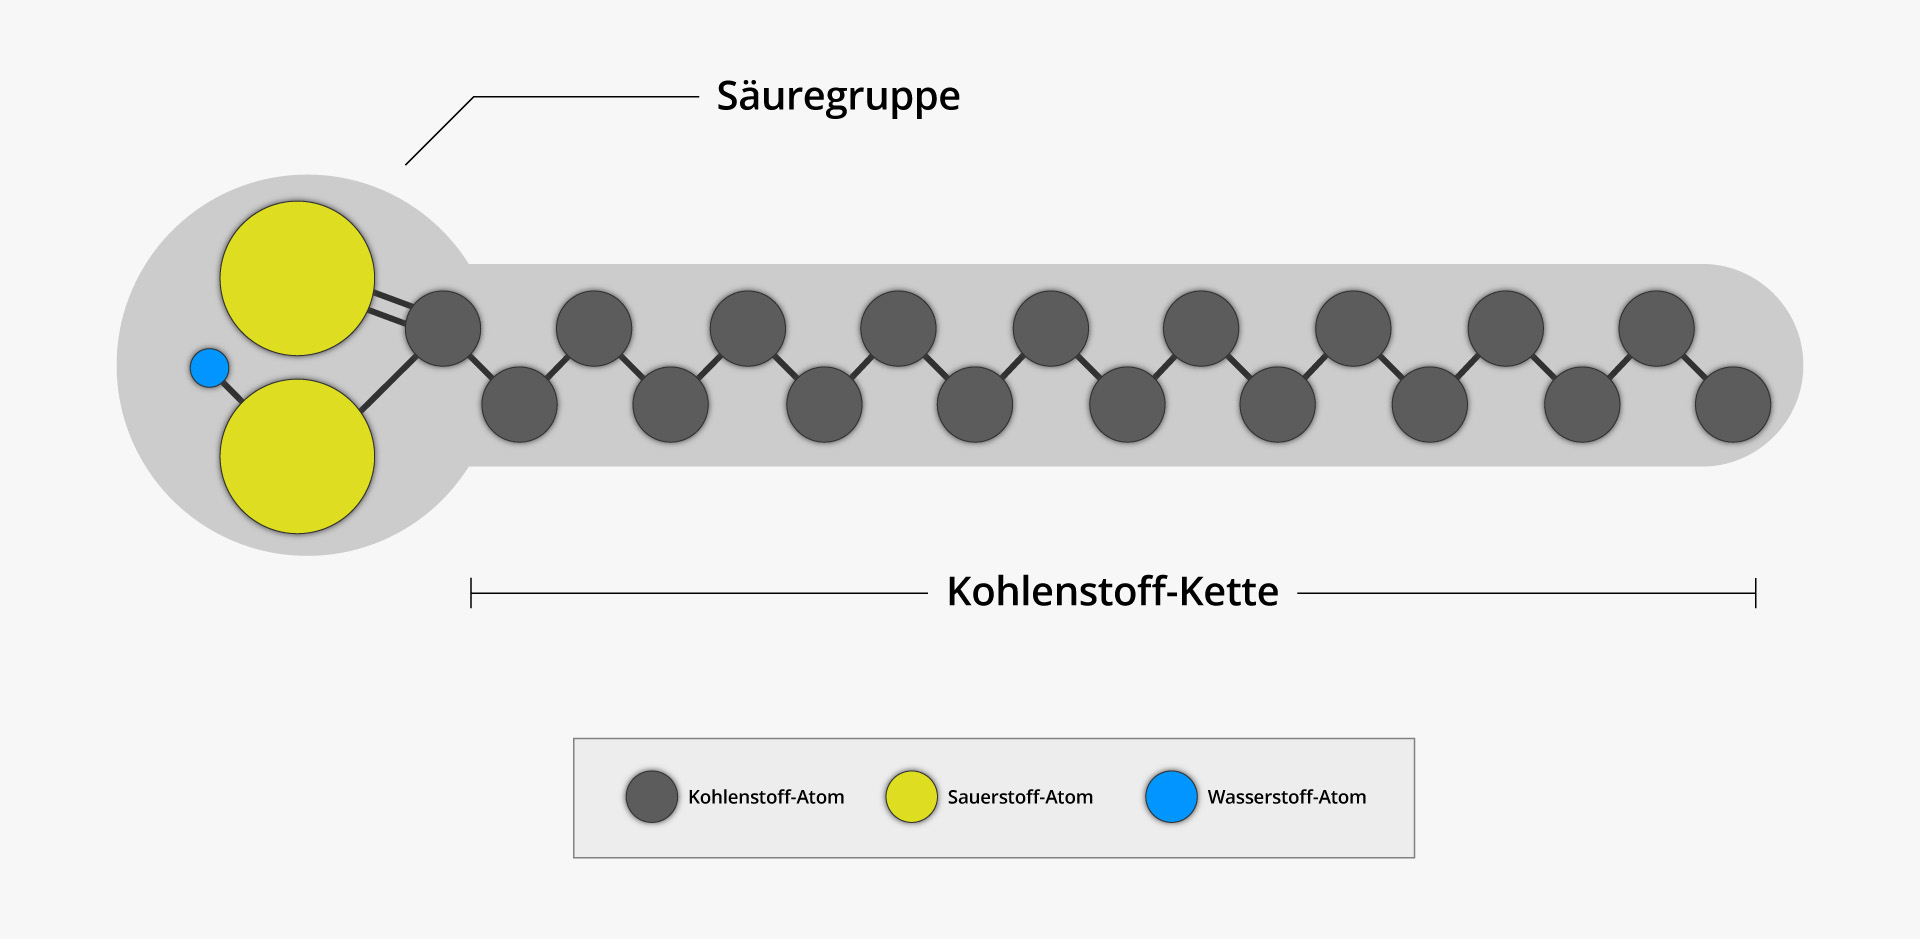
\includegraphics[width=2cm]{../images/fs.png}
            \caption{Fettsäure}
        \end{figure}

        \framebreak

        \begin{figure}
            \centering
            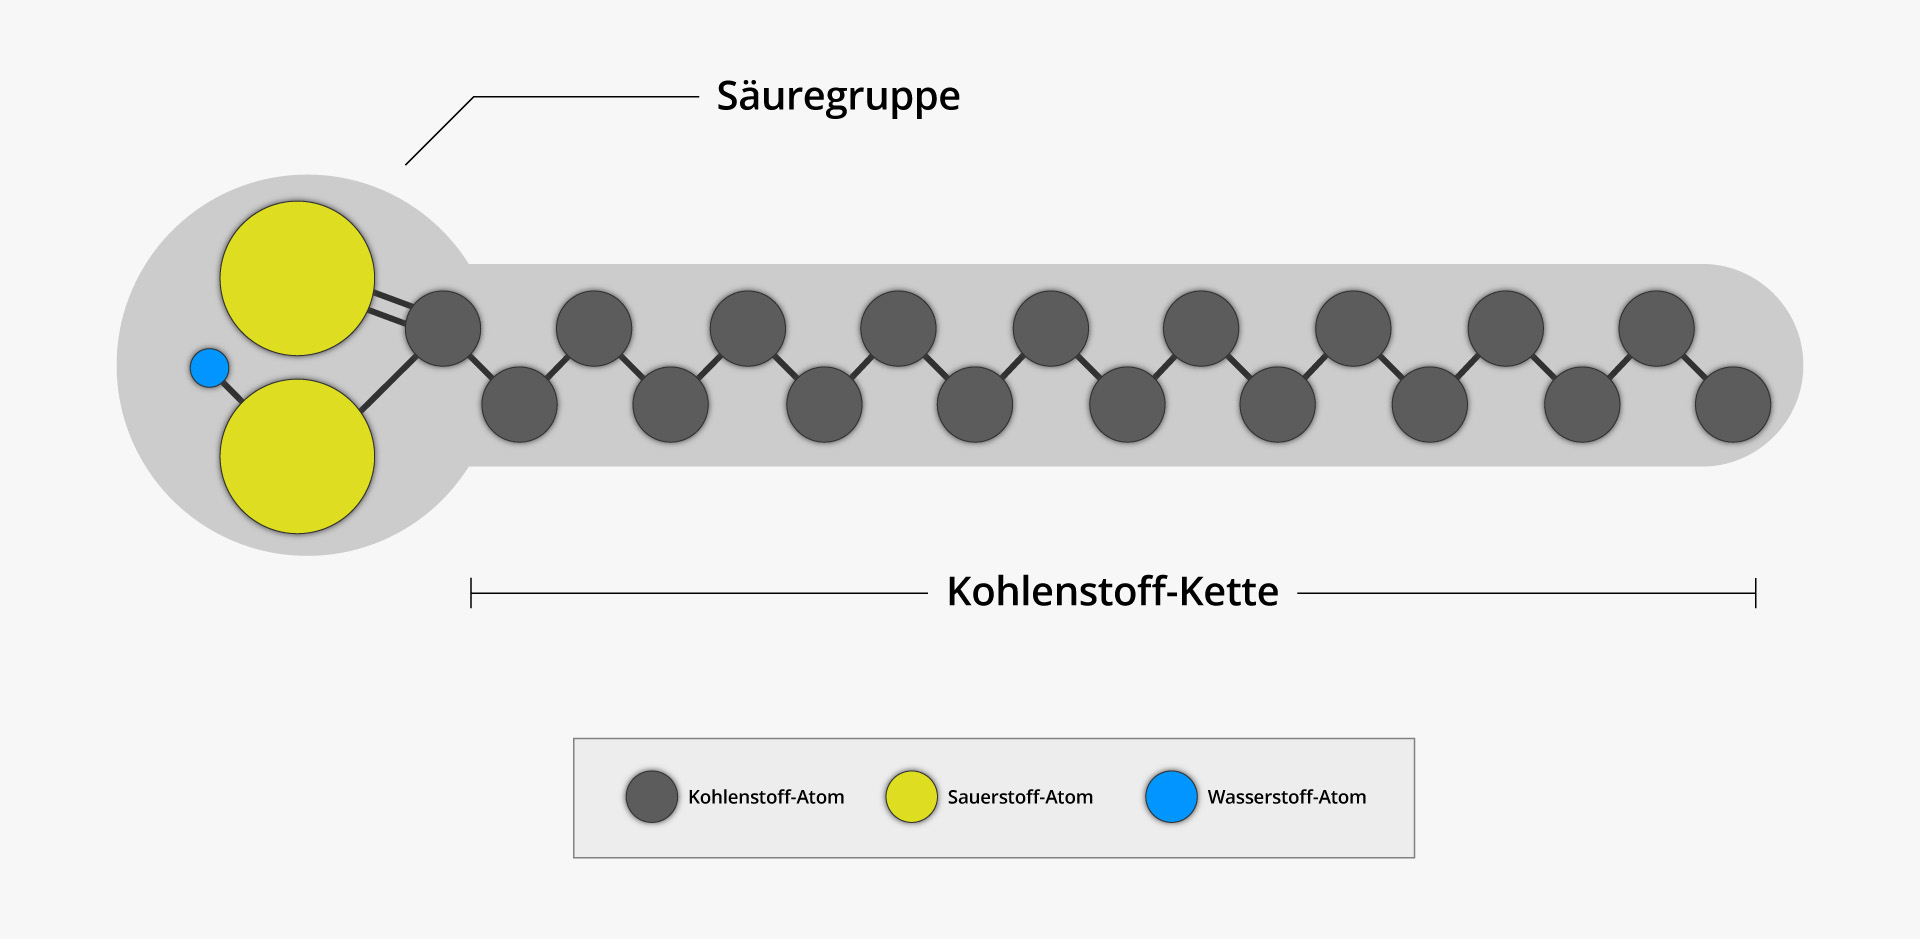
\includegraphics[width=10cm]{../images/fs.jpg}
            \caption{Aufbau von Fettsäuren}
        \end{figure}

        \framebreak

        \begin{figure}
            \centering
            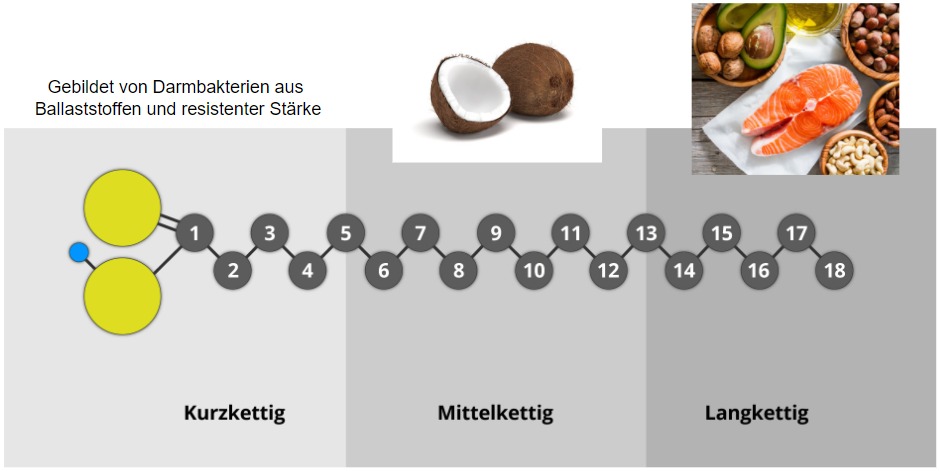
\includegraphics[width=10cm]{../images/fs_2.png}
            \caption{Fettsäuren mit unterschiedlich vielen Kohlenstoffatomen}
        \end{figure}
    \end{frame}

    \subsection{Sättigung}
    \begin{frame}[allowframebreaks]
        \frametitle{Sättigung von Fettsäuren}

        \begin{figure}
            \centering
            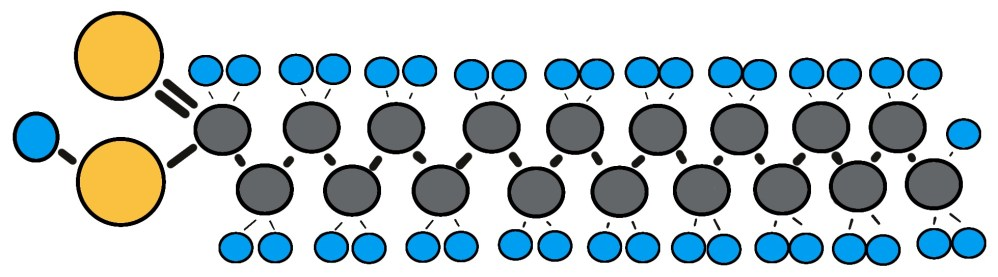
\includegraphics[width=8cm]{../images/fs_3.jpeg}
            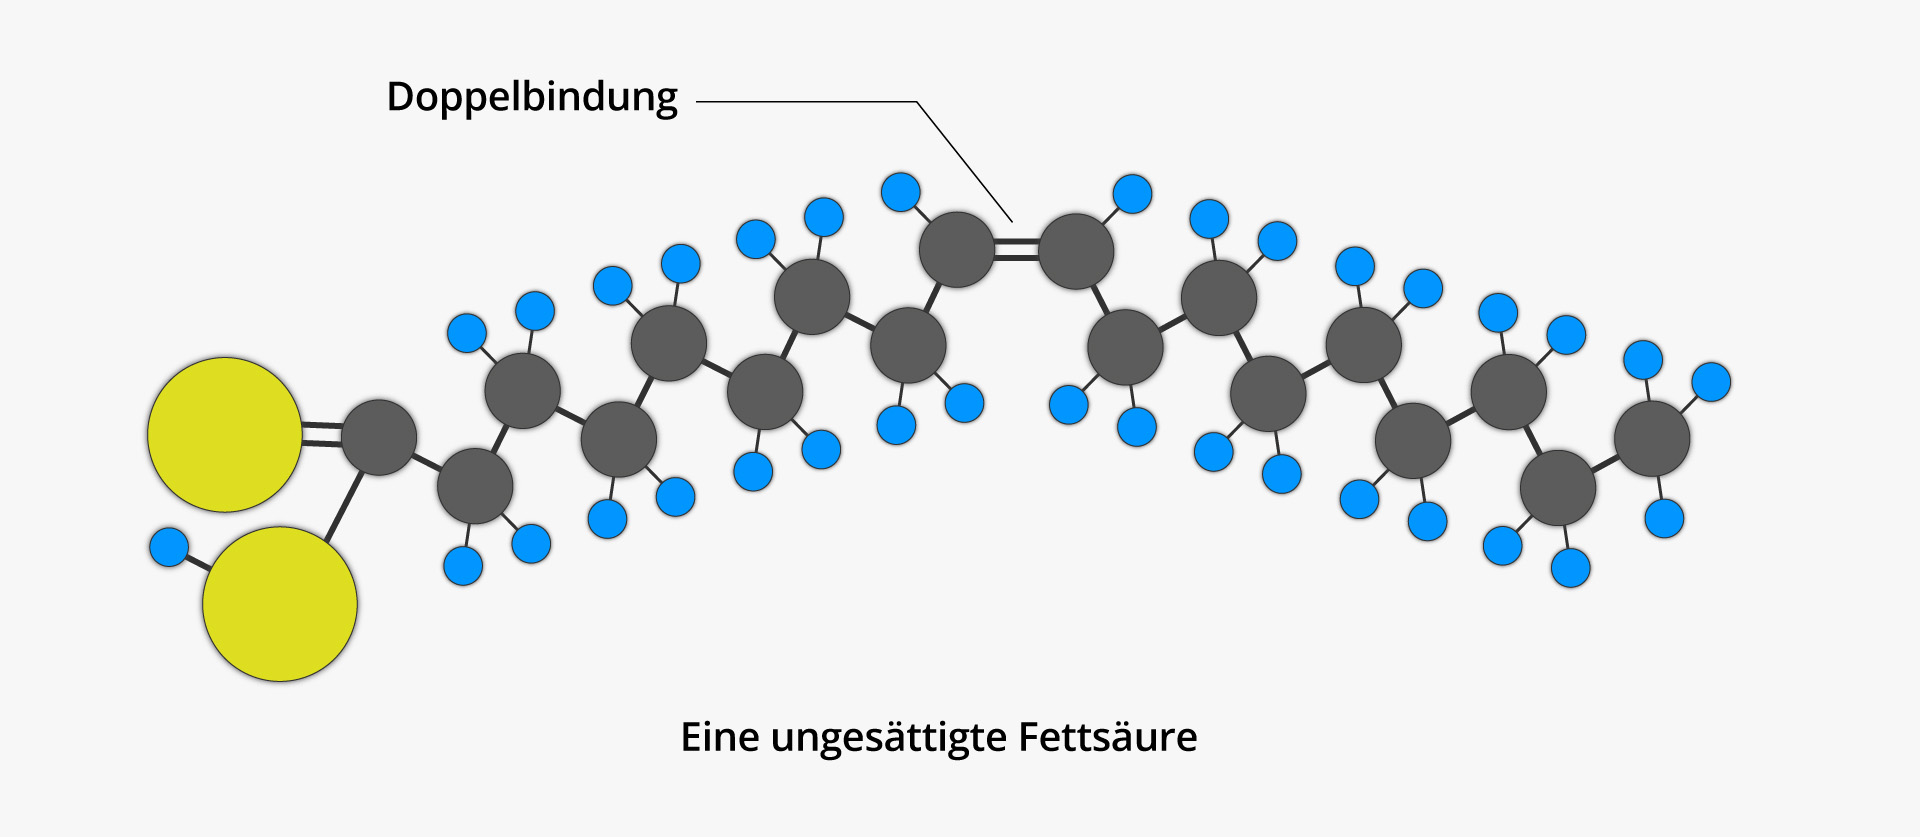
\includegraphics[width=8cm]{../images/fs_4.png}
            \caption{Gesättigte (oben) und ungesättigte (unten) Fettsäure}
        \end{figure}

        \framebreak

        \begin{block}{Gesättigte Fettsäuren \ldots}
            \begin{itemize}
                \setlength\itemsep{1em}
                \item sind bei Raumtemperatur fest (bspw. Butter)
                \item können zu Energie verbrannt werden (einfach ungesättigte FS auch)
                \item können im Fettgewebe gespeichert werden
                \item können selbst hergestellt werden
            \end{itemize}
        \end{block}

        \framebreak

        \begin{block}{Ungesättigte Fettsäuren \ldots}
            \begin{itemize}
                \setlength\itemsep{1em}
                \item sind bei Raumtemperatur flüssig (bspw. Olivenöl)
                \item werden in einfache und mehrfache Un-sättigung eingeteilt
            \end{itemize}
        \end{block}

        \begin{block}{Mehrfach ungesättigte Fettsäuren \ldots}
            \begin{itemize}
                \setlength\itemsep{1em}
                \item werden nicht zu Energie verbrannt
                \item sind Baustoff für Zellwände und Immunstoffe
                \item können nicht vom Körper selbst hergestellt werden
                \item sind lebenswichtige Nährstoffe
                \item werden unterschieden in Omega-3 und Omega-6
            \end{itemize}
        \end{block}

        \framebreak

        \begin{figure}
            \centering
            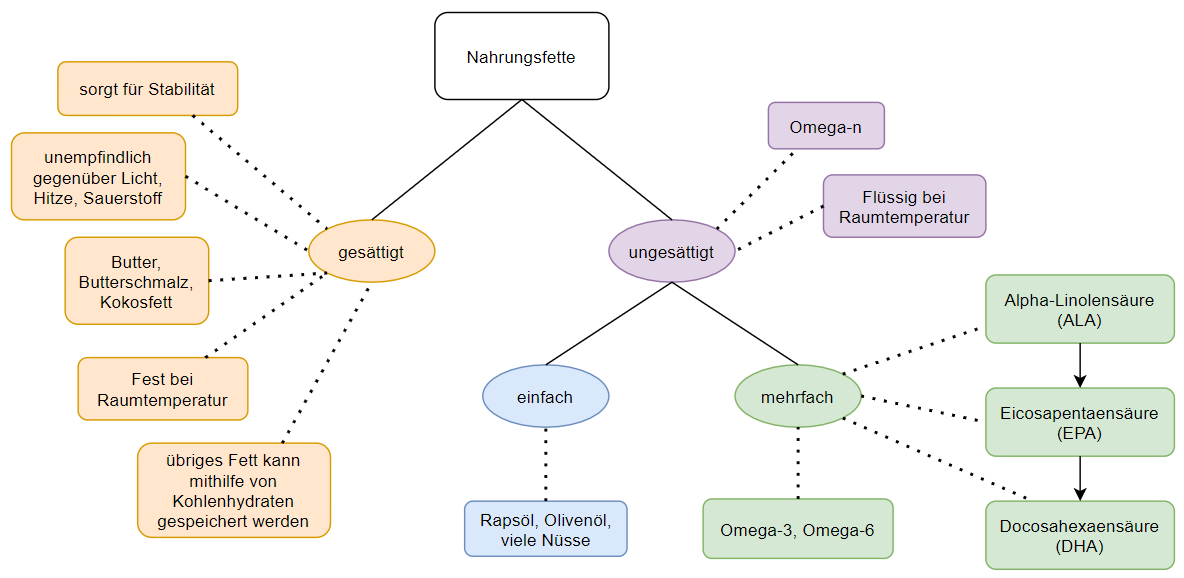
\includegraphics[width=10cm]{../images/nahrungsfette.png}
            \caption{Kategorisierung Nahrungsfette}
        \end{figure}
    \end{frame}

    \subsection{Nahrungsfette}
    \begin{frame}[allowframebreaks]
        \frametitle{Nahrungsfette}

        \begin{figure}
            \centering
            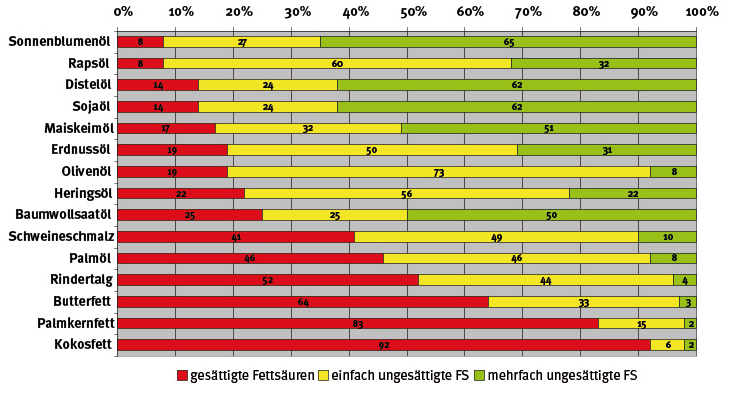
\includegraphics[width=10cm]{../images/fettprofile.png}
            \caption{Fettprofile einiger Lebensmittel}
        \end{figure}

    \end{frame}

    \subsection{Eicosanoide}
    \begin{frame}[allowframebreaks]
        \frametitle{Eicosanoide}

        \begin{block}{Eicosanoide \ldots}
            \begin{itemize}
                \setlength\itemsep{1em}
                \item werden für die Regulierung von Entzündungen gebraucht
                \item sind Botenstoffe des Immunsystems
            \end{itemize}
        \end{block}

        \begin{figure}
            \centering
            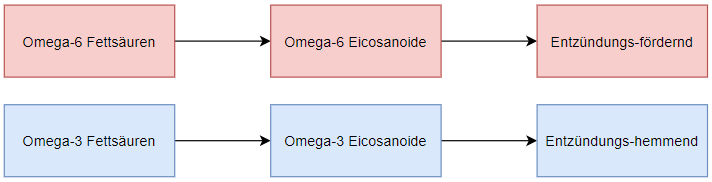
\includegraphics[width=8cm]{../images/eico.png}
            \caption{Verschiedene Eicosanoide}
        \end{figure}

        \framebreak

        \begin{figure}
            \centering
            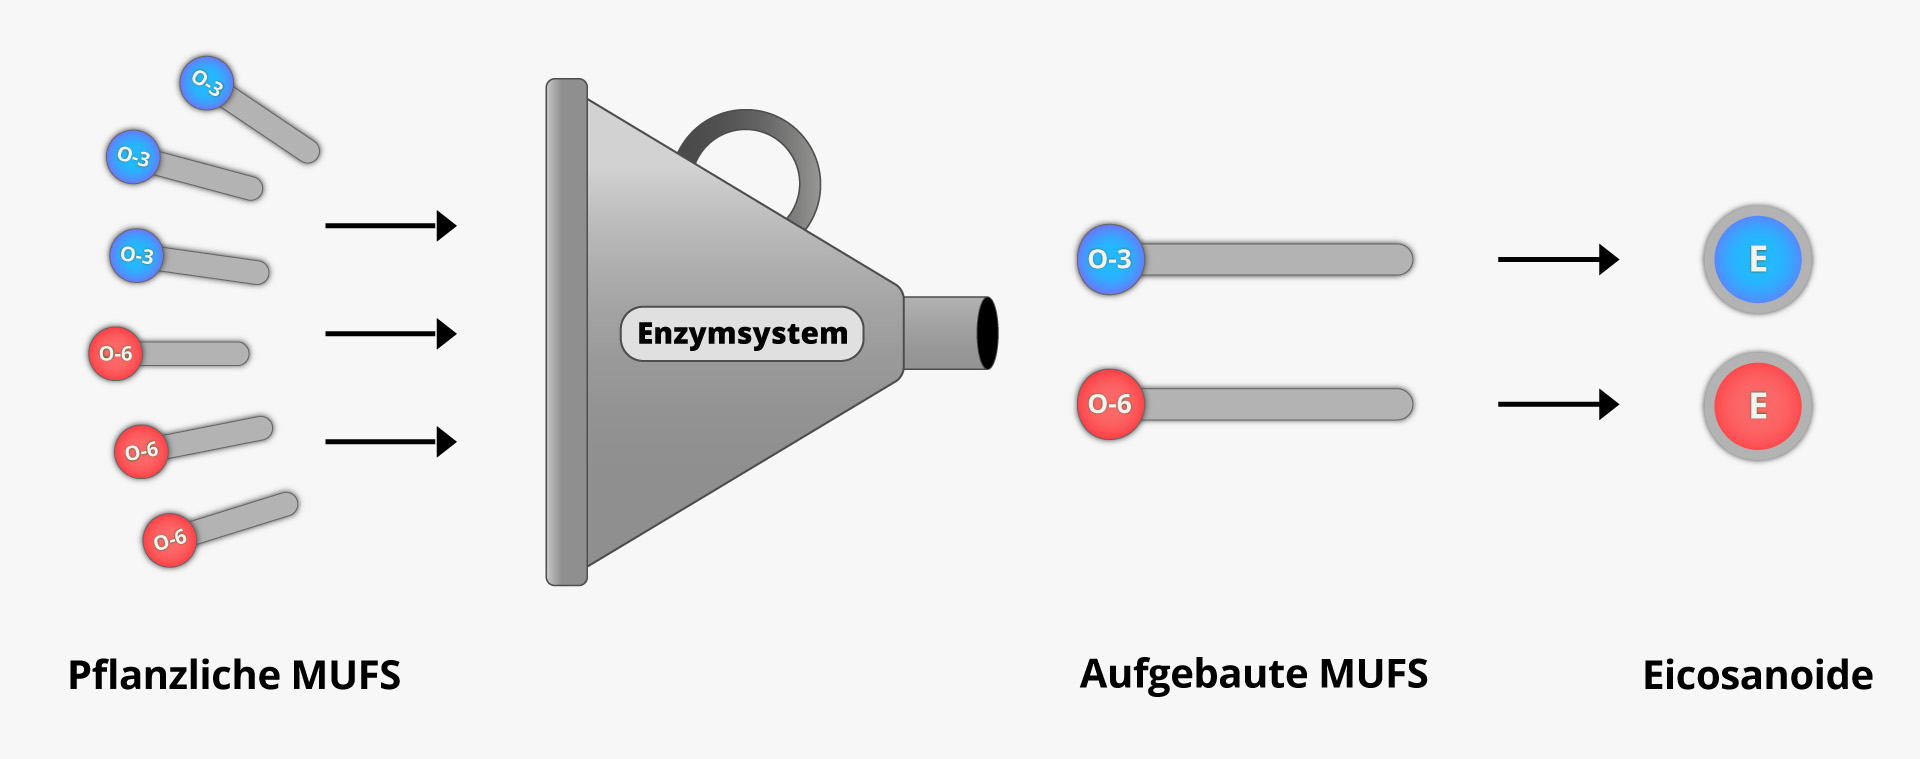
\includegraphics[width=10cm]{../images/eico_1.jpg}
            \caption{Konkurrierender Umbau von Omega-Fettsäuren zu Eicosanoiden}
        \end{figure}

        \framebreak

        \begin{figure}
            \centering
            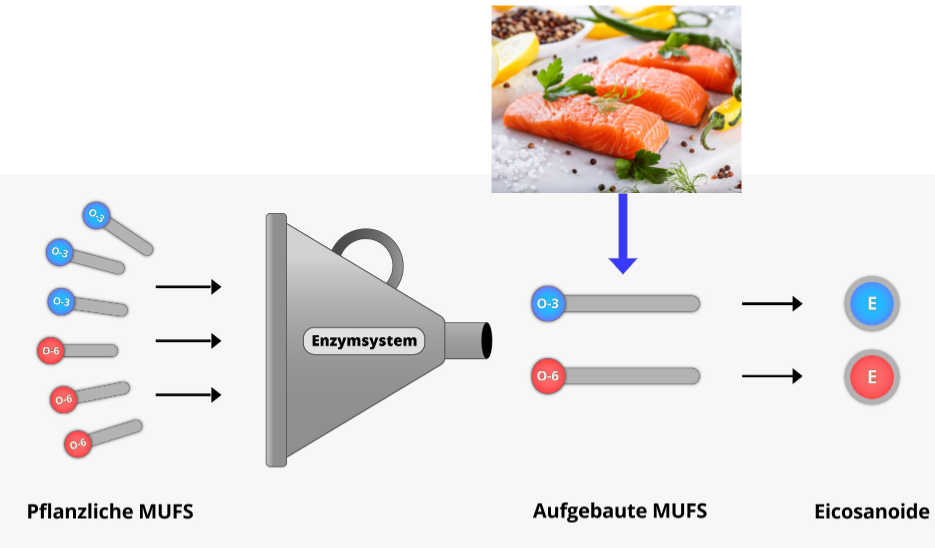
\includegraphics[width=10cm]{../images/eico_2.png}
            \caption{Fetter Seefisch ist besonders wertvoll}
        \end{figure}

    \end{frame}

    \subsection{Nachteile von MUFS}
    \begin{frame}
        \frametitle{Nachteile von MUFS}

        \begin{block}{Mehrfach ungesättigte Fettsäuren \ldots}
            \begin{itemize}
                \setlength\itemsep{1em}
                \item sind sehr reaktionsfreudig
                \item verderben schnell
                \item sind anfällig für Oxidationsprozesse
                \item müssen duch reichlich Antioxidantien geschützt werden
                \item können bei umbedachter Supplementation gefährlich werden (Fischöl-Kapseln)
            \end{itemize}
        \end{block}
    \end{frame}

    \subsection{Tagesbedarf von MUFS}
    \begin{frame}
        \frametitle{Tagesbedarf von MUFS}

        \begin{figure}
            \centering
            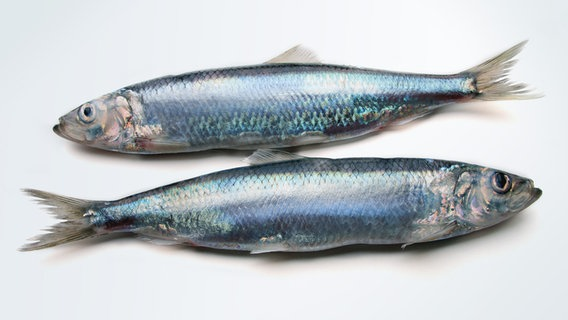
\includegraphics[width=4cm]{../images/hering.jpg}
            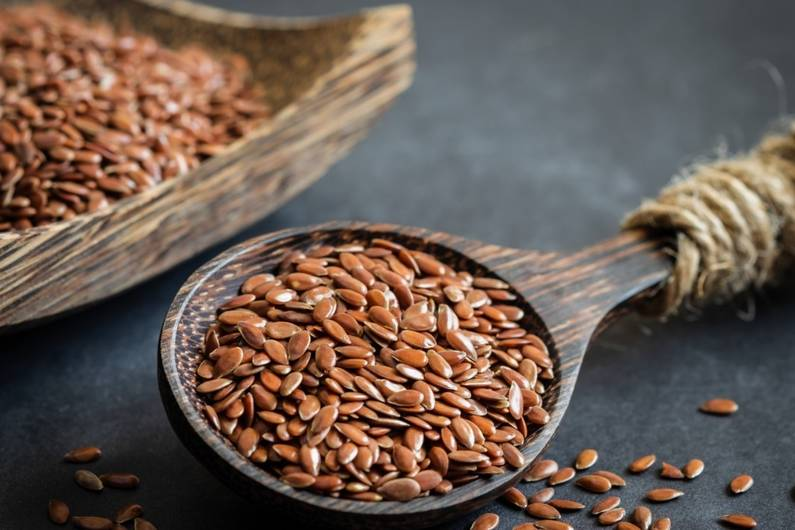
\includegraphics[width=4cm]{../images/leinsamen.jpg}
            \includegraphics[width=4cm]{../images/walnüsse.jpg}
            \caption{40g Hering ODER 10g Leinsamen ODER 20g Walnüsse}
        \end{figure}
    \end{frame}

    \subsection{Cholesterin}
    \begin{frame}[allowframebreaks]
        \frametitle{Cholesterin}

        \begin{block}{Vorteile: Cholesterin \ldots}
            \begin{itemize}
                \setlength\itemsep{1em}
                \item hat fettähnliche Eigenschaften
                \item wird vom Körper selbst hergestellt
                \item baut Zellwände auf
                \item produziert Gallensäure
                \item bildet Hormone
                \item erfüllt also lebenswichtige Aufgaben
            \end{itemize}
        \end{block}

        \framebreak

        \begin{block}{Nachteile: Cholesterin \ldots}
            \begin{itemize}
                \setlength\itemsep{1em}
                \item kann in Wände von Blutgefüßen eindringen, was zur Erkrankung Arteriosklerose führt (echter Nachteil?)
            \end{itemize}
        \end{block}

        \begin{block}{Arteriosklerose \ldots}
            \begin{itemize}
                \setlength\itemsep{1em}
                \item führt zu Herzinfakt
                \item ist die häufigste Todesursache der westlichen Welt
                \begin{itemize}
                    \item jeder zweite Mensch über 65 verstirbt
                    \item jeder dritte Mensch unter 65 verstirbt
                \end{itemize}
            \end{itemize}
        \end{block}

        \begin{figure}
            \centering
            
\includegraphics[width=1cm]{../images/cholesterin.png}
            \caption{Cholesterin}
        \end{figure}

        \framebreak

        \begin{figure}
            \centering
            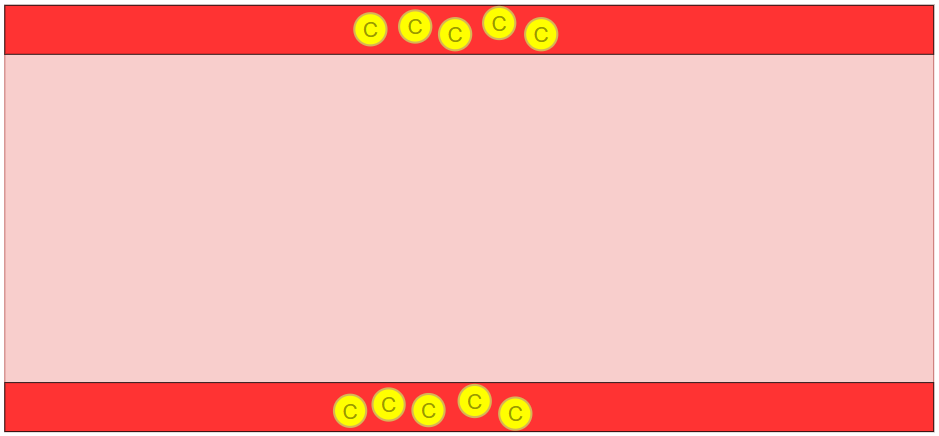
\includegraphics[width=10cm]{../images/ader.png}
            \caption{Blutgefäß mit Gefäßwänden und Cholesterien-Einlagerungen}
        \end{figure}

        \framebreak

        \begin{figure}
            \centering
            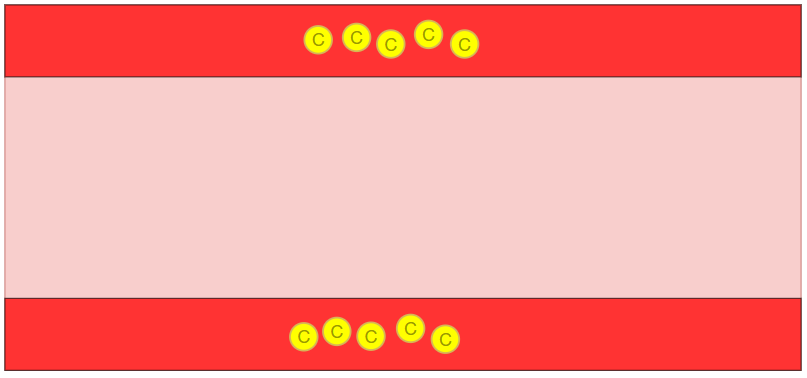
\includegraphics[width=10cm]{../images/ader_2.png}
            \caption{Blutgefäß mit entzündeten Gefäßwänden}
        \end{figure}

        \framebreak

        \begin{figure}
            \centering
            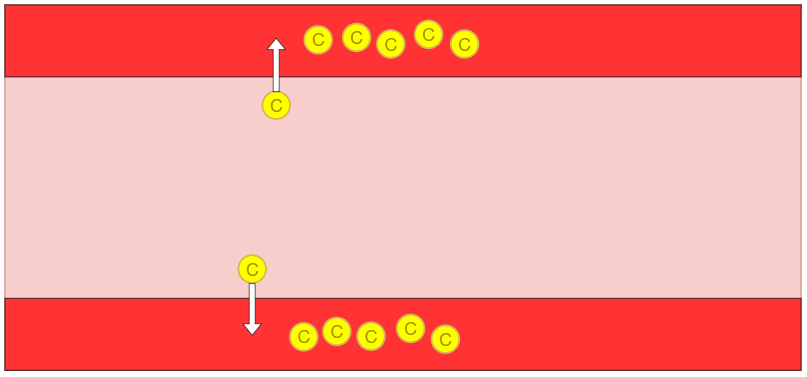
\includegraphics[width=10cm]{../images/ader_3.png}
            \caption{Entzündeten Gefäßwänden werden durchlässiger}
        \end{figure}

        \framebreak

        \begin{figure}
            \centering
            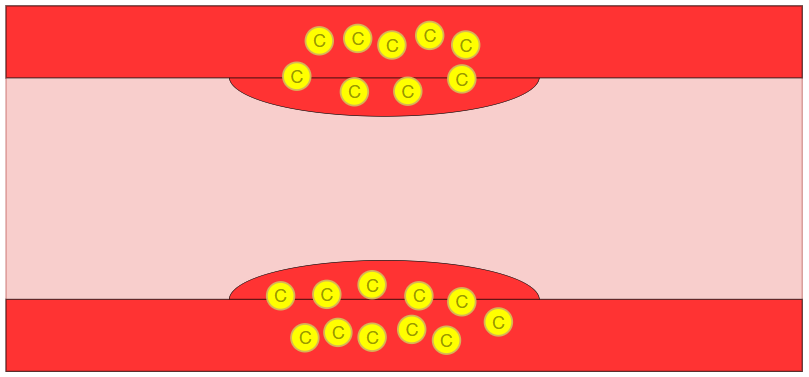
\includegraphics[width=10cm]{../images/ader_4.png}
            \caption{Entzündeten Gefäßwänden werden durchlässiger}
        \end{figure}

        \framebreak

        \begin{block}{Woher kommt das Cholesterin?}
            \begin{itemize}
                \setlength\itemsep{1em}
                \item 50er Jahre: Hoher Cholesterin-Spiegel $\rightarrow$ Cholesterin-Ablagerungen
                \item 60er Jahre: 7-Länder-Studie von Ancel Keys\\ Viele GFS in der Ernährung $\rightarrow$ Hoher Cholesterin-Spiegel
                \item 70er Jahre: Dietary Guidelines (USA, auch DE)\\ Fett- und Cholesterinarme Ernährung $\rightarrow$\\ Energiebedarf aus Kahlenhydraten
                \item 80er Jahre: Nachhaltige Angst vor Cholesterin in der Bevölkerung $\rightarrow$ Butter, Eier, Fleisch wird verteufelt
                \item 90er Jahre: Insulin-Resistenz als neuer Risikofaktor $\rightarrow$ Stellt  40 Jahre Forschung in Frage
            \end{itemize}
        \end{block}

        \framebreak

        \begin{figure}
            \centering
            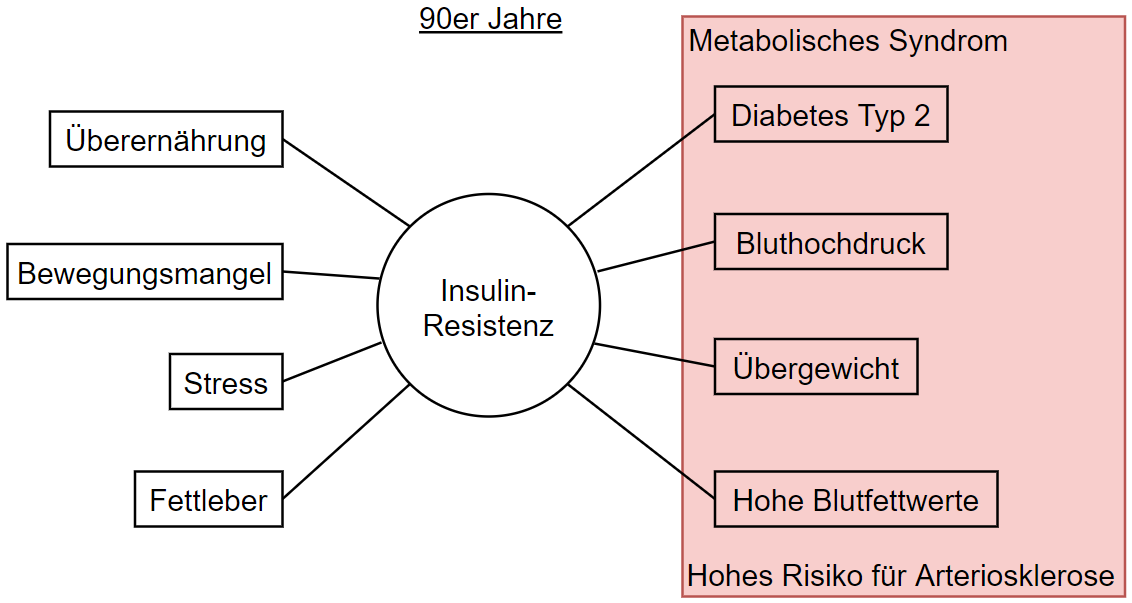
\includegraphics[width=10cm]{../images/90er.png}
            \caption{Forschung 90er Jahre}
        \end{figure}

        \framebreak

        \begin{block}{Heute}
            \begin{itemize}
                \setlength\itemsep{1em}
                \item Moderne Forschung ist einen großen Schritt weiter
                \item Nahrungs-Cholesterin spielt keine Rolle
                \item Cholesterin-Spiegel spielt keine Rolle
                \item Lösung: Lipoproteine
            \end{itemize}
        \end{block}
    \end{frame}

    \subsection{Lioproteine}
    \begin{frame}[allowframebreaks]
        \frametitle{Lioproteine}

        \begin{block}{Lipoproteine \ldots}
            \begin{itemize}
                \setlength\itemsep{1em}
                \item transportieren Fettsäuren durch das Blut
                \item sind sowohl fett- und wasserlöslich
                \item LDL (Low Density Lipoprotein)
                \begin{itemize}
                    \item bringt Cholesterin zu den zellen
                    \item Je kleiner, desto höher die Neigung in Gefäßwände einzudringen
                \end{itemize}
                \item HDL (High Density Lipoprotein)
                \begin{itemize}
                    \item bringt überschüssiges Cholesterin zurück zur Leber
                \end{itemize}
            \end{itemize}
        \end{block}

        \begin{figure}
            \centering
            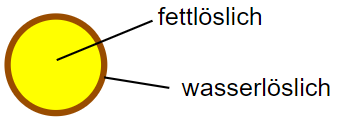
\includegraphics[width=2cm]{../images/lipo.png}
            \caption{Lipoprotein}
        \end{figure}

        \framebreak

        \begin{figure}
            \centering
            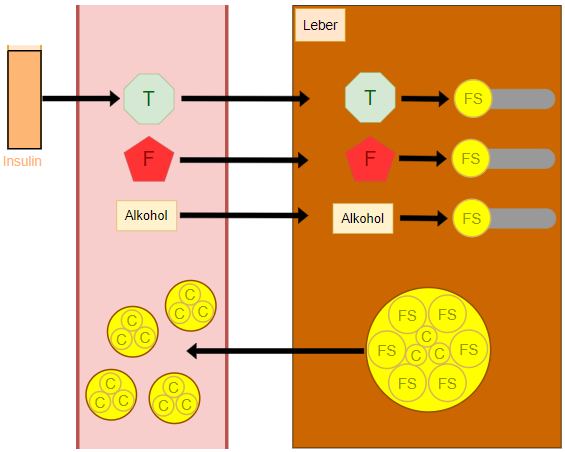
\includegraphics[width=7cm]{../images/lipo_1.png}
            \caption{Herstellung von Lipoproteinen einer gestressten Leber}
        \end{figure}

    \end{frame}

    \section{Praxis}
    {
        \setbeamercolor{normal text}{fg=hBlue}\usebeamercolor*{normal text}
        \begin{frame}
            \begin{center}
                \Huge Praxis
            \end{center}
        \end{frame}
    }

    \begin{frame}{Tipps \& Tricks}
        \begin{itemize}
            \setlength\itemsep{1em}
            \item Omega-6 reiche Nahrungsmittel redizieren
            \begin{itemize}
                \item Reaffinierte Pflanzenöle, wie Sonnenblumenöl, Maiskeimöl, etc.
                \item Magarine
                \item Fertigprodukte (vor allem Backwaren)
            \end{itemize}
            \item Omega-3 reiche Nahrungsmittel gezielt in die Ernährungs einbauen
            \begin{itemize}
                \item Fetter Seefisch, wie Lachs, Makrele, etc.
                \item Leinsamen
                \item Nüsse, wie Walnüsse, Haselnüsse, etc.
            \end{itemize}
            \item Leber-Stress reduzieren / Gefährliche Lebensstilfaktoren verringern
            \begin{itemize}
                \item Überernährung mit Kohlenhydraten
                \item Bewegungsmangel
                \item Stress
                \item Fettleber
            \end{itemize}
            \item Das "`perfekte'" Früchstück ;)
        \end{itemize}
    \end{frame}

    \section{Fragerunde}
    {
        \setbeamercolor{normal text}{fg=hBlue}\usebeamercolor*{normal text}
        \begin{frame}
            \begin{center}
                \Huge Fragerunde
            \end{center}
        \end{frame}
    }

\end{document}